 \chapter{Risultati computazionali} \label{chap:risultati}

% **************************** Define Graphics Path **************************
\ifpdf
    \graphicspath{{Chapter7/Figs/Raster/}{Chapter7/Figs/PDF/}{Chapter7/Figs/}}
\else
    \graphicspath{{Chapter7/Figs/Vector/}{Chapter7/Figs/}}
\fi

\section{Costruzione del dataset}
Abbiamo preso in considerazione due tipologie di istanze, basate sui set di posizioni potenziali $P$ e illustrate in \figurename\ \ref{figP}, rappresentanti diversi scenari. \\
La prima tipologia consiste in griglie quadrate o rettangolari $LxH$ (lunghezza x altezza, in numero di punti) complete, ovvero in cui in ogni punto interno è possibile posizionare un drone. Le griglie rettangolari, soprattutto se $L << H$ (o viceversa), si rivelano particolarmente interessanti in quanto permettono la costruzione di vere e proprie "catene" di droni. La seconda tipologia invece (griglie "bottleneck" $btn25$, $btn41$, $btn48$ \cite{degioPal2013}, dove 25, 41 e 48 sono il numero di posizioni ammissibili) include posizioni vietate, dette no-flight zones, causate per esempio da ostacoli o divieti di sorvolo. Queste particolari configurazioni vengono implementate costruendo la griglia completa e successivamente ponendo a 0 il valore minimo e massimo del dominio delle variabili $y_i$ corrispondenti a posizioni vietate.\\
%
\begin{figure}
	\begin{center}
		\includegraphics[scale=0.60]{figTopolHorUsersP}
	\end{center}
	\caption{Tipologie di griglie utilizzate.} \label{figP}
\end{figure}
%
Le posizioni degli utenti sono state generate in maniera casuale attorno all'area della griglia, con maggiore probabilità attorno ai bordi (ad esempio, le croci blu in \figurename\ \ref{figP}), assicurandosi che tutti i client si trovassero a distanze minori di $R$ da ciascun punto $i \in P$, per evitare istanze impossibili da risolvere a causa del cattivo posizionamento. \\
Test preliminari per il dimensionamento del dataset hanno dimostrato l'impossibilità di risolvere istanze, con i vincoli temporali e di memoria stabiliti, con un numero di clients $n \geq 30$. \\
Le griglie "complete" impiegate nel dataset, identificate dalla loro dimensione(lunghezza x altezza, in numero di punti) sono le seguenti: 4x8, 6x6, 9x9, 5x10, 6x15, 8x20. Oltre a queste, come già accennato, sono state utilizzate le griglie "speciali" $btn25$, $btn41$, $btn48$.\\
Per ogni griglia e per ogni numero di utenti nell'insieme $\{5, 10, 15, 20, 25, 30\}$ sono state generate 3 istanze casuali, generando in maniera casuale le posizioni degli utenti e le matrici di traffico. \\

\subsection{Relazione tra dimensione delle istanze e tempi di esecuzione}
Nella fase di dimensionamento del dataset abbiamo cercato di identificare quali parametri, di una generica istanza, influissero maggiormente sui tempi di esecuzione di CPLEX, e in che maniera:
\begin{itemize}
	\item Il numero di client influisce notevolmente sulle dimensioni del modello, in quanto da esso dipende direttamente il numero di commodities dell'istanza ($|K| = n(n-1)$), e di conseguenza il numero di variabili $f_{ij}^{sd}$ generate, il numero di vincoli di flusso (\ref{eq:balance}) e il numero di termini dei vincoli (\ref{eq:capTX}) e (\ref{eq:capRX}); 
	\item Il numero di punti della griglia è un altro fattore decisivo per i tempi di esecuzione, poiché la cardinalità dell'insieme di posizioni potenziali $P$ è direttamente proporzionale al numero totale di vincoli generati dal modello;
	\item Il range trasmissivo dei nodi (sia droni che client) influenza la cardinalità dell'insieme di variabili $f_{ij}^{sd}$, in quanto vengono generate solo quelle tali che $d(i,j) \leq R$, e il numero di termini delle sommatorie nei vincoli (\ref{eq:setSub}) e (\ref{eq:setSlb}), in quanto dipendenti dal numero di posizioni potenziali nel range di ciascun nodo. 
\end{itemize} 

\section{Risultati}
Come detto nel \chaptername\ \ref{cap:metodi}, il modello è stato implementato in C++ utilizzando le CPLEX Callable Library (C API), con tempo massimo di esecuzione di 2400 secondi (40 minuti), parallelismo deterministico e focus sull'ottimizzazione della memoria. Per le griglie si è utilizzato uno step di 5m (inteso come distanza, in metri, tra due punti adiacenti) e ai nodi è stato assegnato un range trasmissivo $R = 50m$ e una area critica di raggio $R_\epsilon = 15m$. \\
Le istanze sono state risolte su un sistema con 4 processori Intel Xeon E5520 @2.27 GHz e 32 GB di RAM. \\

\subsection{Risultati con metodi esatti} \label{sec:esatti}
I risultati ottenuti elaborando il dataset con CPLEX v12.6.0 sono mostrati in \tablename\ \ref{tab:esatto}.
Ogni riga contiene i dati aggregati dell'esecuzione di tre istanze per ogni combinazione griglia-client. \\
Le prime due colonne indicano il nome della griglia e il numero di client che vi sono stati posizionati casualmente. Le colonne AVG(sec), MIN(sec) e MAX(sec) indicano, rispettivamente, il tempo medio, minimo e massimo per ottenere la soluzione ottima, espresso in secondi. AVG(UAV) indica il numero medio di droni richiesti dalle istanze, mentre AVG(gap) indica il gap medio relativo tra il valore ottimo della funzione obbiettivo e il suo migliore bound noto tra tutti i nodi aperti rimanenti. Quando un problema viene risolto all'ottimo, il best bound coincide con valore della soluzione, e il gap varrà quindi 0. Infine, la colonna \# end indica quante istanze, sul totale per ogni combinazione griglia-client, sono state risolte all'ottimo entro il tempo limite. \\
Si può notare che, a parità di griglia, ad ogni incremento del numero di client si ha un aumento di circa un ordine di grandezza dei tempi per trovare la soluzione ottima. 
Lo stesso aumento si può notare al raddoppiare del numero di punti della griglia. Per poter risolvere all'ottimo istanze fino a 30 utenti è necessario impiegare griglie sufficientemente piccole, al di sotto dei 25-30 punti. \\
All'interno di ogni combinazione griglia-client il valore della funzione obbiettivo, cioè il numero di droni posizionati, si dimostra pressoché stabile, con variazioni medie di 0-1 unità. Il numero di droni è generalmente basso (ad eccezione delle istanze in cui non viene trovata una soluzione entro il limite temporale) in quanto il range di 50m selezionato offre un'ampia copertura rispetto la dimensione media delle griglie. Ridurre il range, aumentare la dimensione della griglia o la sua grana sono espedienti che possono essere utilizzati per incrementare il numero medio di droni impiegato.\\
Anche l'incremento degli utenti causa un aumento medio nel numero di droni a causa della maggior banda richiesta. \\ 
%
\setlength{\tabcolsep}{3.5 pt}
\renewcommand\arraystretch{1.1}
\begin{table}[]
	\centering
	\scriptsize
	\begin{tabular}{@{}llllllll@{}}
		\toprule
		Griglia & Utenti & AVG (sec) & MIN (sec) & MAX (sec) & AVG (UAV)  & AVG (gap) & \# end \\ \midrule
		4x8     & 5             & 0,7           & 0,5         & 0,9         & 1          & 0,0     & 3          \\
		4x8     & 10            & 14,0          & 11,9        & 15,6        & 4          & 0,0     & 3          \\
		4x8     & 15            & 71,7          & 56,0        & 87,7        & 3          & 0,0     & 3          \\
		4x8     & 20            & 281,5         & 181,4       & 397,3       & 11         & 0,0     & 3          \\
		4x8     & 25            & 1394,7        & 1051,1      & 1779,0      & 7          & 0,0     & 3          \\
		4x8     & 30            & 2400,0        & 2400,0      & 2400,0      & 32         & 1,0     & 0          \\
		5x10    & 5             & 1,6           & 1,6         & 1,7         & 1          & 0,0     & 3          \\
		5x10    & 10            & 38,9          & 30,9        & 44,7        & 4          & 0,0     & 3          \\
		5x10    & 15            & 285,6         & 265,1       & 304,5       & 3          & 0,0     & 3          \\
		5x10    & 20            & 965,3         & 923,5       & 995,9       & 16         & 0,0     & 3          \\
		5x10    & 25            & 2401,3        & 2400,8      & 2402,0      & 50         & 0,9     & 0          \\
		5x10    & 30            & 2400,6        & 2400,5      & 2400,6      & 50         & 1,0     & 0          \\
		6x15    & 5             & 14,3          & 12,2        & 17,3        & 2          & 0,0     & 3          \\
		6x15    & 10            & 455,6         & 347,8       & 611,4       & 5          & 0,0     & 3          \\
		6x15    & 15            & 1550,1        & 1019,7      & 2400,7      & 4          & 0,1     & 2          \\
		6x15    & 20            & 2400,8        & 2400,5      & 2401,4      & 90         & 0,9     & 0          \\
		6x15    & 25            & 2400,6        & 2400,6      & 2400,6      & 90         & 1,0     & 0          \\
		6x15    & 30            & 2400,0        & 2400,0      & 2400,0      & 90         & 1,0     & 0          \\
		6x6     & 5             & 0,7           & 0,7         & 0,8         & 1          & 0,0     & 3          \\
		6x6     & 10            & 13,8          & 12,8        & 14,5        & 4          & 0,0     & 3          \\
		6x6     & 15            & 143,2         & 104,3       & 214,2       & 3          & 0,0     & 3          \\
		6x6     & 20            & 411,5         & 393,0       & 442,1       & 16         & 0,0     & 3          \\
		6x6     & 25            & 1466,3        & 1283,7      & 1581,0      & 7          & 0,0     & 3          \\
		6x6     & 30            & 2400,7        & 2400,4      & 2401,2      & 36         & 0,8     & 0          \\
		8x20    & 5             & 125,2         & 71,9        & 223,3       & 2          & 0,0     & 3          \\
		8x20    & 10            & 2352,8        & 2256,5      & 2401,4      & 29         & 0,6     & 1          \\
		8x20    & 15            & 2403,0        & 2400,7      & 2407,3      & 118        & 1,0     & 0          \\
		8x20    & 20            & 2403,9        & 2402,2      & 2406,0      & 157        & 1,0     & 0          \\
		8x20    & 25            & 2400,0        & 2400,0      & 2400,0      & 160        & 1,0     & 0          \\
		8x20    & 30            & 2400,0        & 2400,0      & 2400,0      & 160        & 1,0     & 0          \\
		9x9     & 5             & 9,7           & 6,1         & 12,3        & 1          & 0,0     & 3          \\
		9x9     & 10            & 210,4         & 139,6       & 282,7       & 4          & 0,0     & 3          \\
		9x9     & 15            & 1444,1        & 1087,0      & 2053,4      & 3          & 0,0     & 3          \\
		9x9     & 20            & 2400,7        & 2400,5      & 2401,0      & 80         & 1,0     & 0          \\
		9x9     & 25            & 2400,6        & 2400,6      & 2400,7      & 81         & 1,0     & 0          \\
		9x9     & 30            & 2400,0        & 2400,0      & 2400,0      & 81         & 1,0     & 0          \\
		btn25   & 5             & 0,6           & 0,4         & 0,7         & 1          & 0,0     & 3          \\
		btn25   & 10            & 6,3           & 6,0         & 6,7         & 2          & 0,0     & 3          \\
		btn25   & 15            & 42,2          & 31,6        & 52,7        & 3          & 0,0     & 3          \\
		btn25   & 20            & 150,5         & 136,8       & 172,4       & 5          & 0,0     & 3          \\
		btn25   & 25            & 541,7         & 498,0       & 576,1       & 7          & 0,0     & 3          \\
		btn25   & 30            & 1193,6        & 976,5       & 1343,8      & 10         & 0,0     & 3          \\
		btn41   & 5             & 2,3           & 1,8         & 2,6         & 2          & 0,0     & 3          \\
		btn41   & 10            & 33,7          & 31,8        & 36,7        & 2          & 0,0     & 3          \\
		btn41   & 15            & 903,4         & 198,3       & 2234,0      & 4          & 0,0     & 3          \\
		btn41   & 20            & 816,1         & 332,5       & 1190,1      & 6          & 0,0     & 3          \\
		btn41   & 25            & 1908,9        & 1640,1      & 2219,2      & 8          & 0,0     & 3          \\
		btn41   & 30            & 2401,1        & 2400,7      & 2401,6      & 43         & 0,7     & 0          \\
		btn48   & 5             & 2,5           & 1,7         & 3,1         & 1          & 0,0     & 3          \\
		btn48   & 10            & 39,7          & 36,9        & 42,7        & 4          & 0,0     & 3          \\
		btn48   & 15            & 236,9         & 219,6       & 258,6       & 3          & 0,0     & 3          \\
		btn48   & 20            & 2370,7        & 2308,9      & 2401,9      & 23         & 0,2     & 1          \\
		btn48   & 25            & 2204,7        & 1812,2      & 2401,0      & 31         & 0,4     & 1          \\
		btn48   & 30            & 2400,2        & 2400,0      & 2400,7      & 48         & 1,0     & 0          \\ \bottomrule
	\end{tabular}
	\caption{Risultati dataset risolto con CPLEX v12.6.0}
	\label{tab:esatto}
\end{table}
%
\subsection{Risultati con metodi euristici}
In \tablename\ \ref{tab:euristica} sono mostrati i risultati ottenuti tramite gli algoritmi euristici descritti nella sezione \ref{sec:euristica}. Oltre alle colonne precedentemente descritte in sezione \ref{sec:esatti}, la colonna AVG(itr.) indica il numero medio di iterazioni compiuti dall'algoritmo euristico per trovare la soluzione ottima. \\
Dal punto di vista temporale, l'euristica Set Y impiega generalmente meno tempo a trovare la soluzione ottima rispetto alla Binary Y: considerando le sole istanze che hanno fornito una soluzione ottima entro il time limit, Set Y impiega un tempo minore circa il 63\% delle volte. 
Le differenze delle tempistiche sembrano essere molto variabili, entro un range del 15\%-70\%. \\
Una delle possibili cause può essere data dal fatto che l'algoritmo Set Y, ad ogni iterazione, cerca di risolvere il problema MIP solamente se il rilassamento continuo, generalmente molto più veloce, ha fornito una soluzione, risparmiando così tempo di elaborazione qualora non ci fosse. Riformulando l'algoritmo Binary Y potrebbe essere possibile migliorarne fortemente le performance temporali.   \\
Per quanto riguarda invece la precisione della soluzione, ovvero il numero di droni minimo necessario, se si escludono tutte le istanze che non hanno saputo trovare la soluzione ottima entro il tempo limite, non si notano differenze rilevanti tra i due algoritmi, in quanto lo scarto tende a essere compreso tra 0 e 2 droni. 
%
\begin{table}[]
	\centering
	\scriptsize
	\begin{tabular}{llllllllllllllll}
		\hline
		&        & \multicolumn{7}{l}{Set Y}                                                                                                                                                                                                                                                                                                                        & \multicolumn{7}{l}{Binary Y}                                                                                                                                                                                                                                                                                                                     \\ \hline
		Griglia & Utenti & \begin{tabular}[c]{@{}l@{}}AVG\\ (sec)\end{tabular} & \begin{tabular}[c]{@{}l@{}}MIN\\ (sec)\end{tabular} & \begin{tabular}[c]{@{}l@{}}MAX\\ (sec)\end{tabular} & \begin{tabular}[c]{@{}l@{}}AVG\\ (UAV)\end{tabular} & \begin{tabular}[c]{@{}l@{}}AVG\\ (gap)\end{tabular} & \# end & \begin{tabular}[c]{@{}l@{}}AVG\\ (itr.)\end{tabular} & \begin{tabular}[c]{@{}l@{}}AVG\\ (sec)\end{tabular} & \begin{tabular}[c]{@{}l@{}}MIN\\ (sec)\end{tabular} & \begin{tabular}[c]{@{}l@{}}MAX\\ (sec)\end{tabular} & \begin{tabular}[c]{@{}l@{}}AVG\\ (UAV)\end{tabular} & \begin{tabular}[c]{@{}l@{}}AVG\\ (gap)\end{tabular} & \# end & \begin{tabular}[c]{@{}l@{}}AVG\\ (itr.)\end{tabular} \\
		4x8     & 5      & 0,6                                                 & 0,5                                                 & 0,6                                                 & 3                                                   & 0,0                                                 & 3      & 3                                                         & 1,4                                                 & 1,3                                                 & 1,5                                                 & 3                                                   & 0,0                                                 & 3      & 4                                                         \\
		4x8     & 10     & 8,2                                                 & 7,9                                                 & 8,5                                                 & 5                                                   & 0,0                                                 & 3      & 5                                                         & 13,1                                                & 9,8                                                 & 15,5                                                & 5                                                   & 0,0                                                 & 3      & 4                                                         \\
		4x8     & 15     & 65,9                                                & 60,9                                                & 71,7                                                & 3                                                   & 0,0                                                 & 3      & 3                                                         & 89,0                                                & 84,3                                                & 92,5                                                & 3                                                   & 0,0                                                 & 3      & 4                                                         \\
		4x8     & 20     & 307,3                                               & 283,9                                               & 321,9                                               & 11                                                  & 0,0                                                 & 3      & 11                                                        & 487,8                                               & 388,7                                               & 594,2                                               & 11                                                  & 0,0                                                 & 3      & 5                                                         \\
		4x8     & 25     & 1194,9                                              & 737,8                                               & 1970,0                                              & 7                                                   & 0,0                                                 & 3      & 7                                                         & 638,9                                               & 583,0                                               & 716,3                                               & 7                                                   & 0,0                                                 & 3      & 4                                                         \\
		4x8     & 30     & 2400,0                                              & 2400,0                                              & 2400,0                                              & 32                                                  & 1,0                                                 & 0      & 17                                                        & 2400,0                                              & 2400,0                                              & 2400,0                                              & 32                                                  & 1,0                                                 & 0      & 4                                                         \\
		5x10    & 5      & 1,4                                                 & 1,4                                                 & 1,5                                                 & 1                                                   & 0,0                                                 & 3      & 1                                                         & 3,8                                                 & 3,3                                                 & 4,8                                                 & 2                                                   & 0,0                                                 & 3      & 5                                                         \\
		5x10    & 10     & 47,6                                                & 46,3                                                & 48,6                                                & 4                                                   & 0,0                                                 & 3      & 4                                                         & 39,9                                                & 38,8                                                & 40,5                                                & 4                                                   & 0,0                                                 & 3      & 4                                                         \\
		5x10    & 15     & 250,2                                               & 225,6                                               & 264,0                                               & 5                                                   & 0,0                                                 & 3      & 5                                                         & 275,3                                               & 235,1                                               & 315,1                                               & 5                                                   & 0,0                                                 & 3      & 5                                                         \\
		5x10    & 20     & 686,3                                               & 541,1                                               & 927,9                                               & 17                                                  & 0,0                                                 & 3      & 17                                                        & 862,6                                               & 716,4                                               & 964,6                                               & 17                                                  & 0,0                                                 & 3      & 5                                                         \\
		5x10    & 25     & 2400,4                                              & 2400,0                                              & 2400,2                                              & 36                                                  & 0,7                                                 & 1      & 27                                                        & 2225,7                                              & 1877,0                                              & 2400,0                                              & 21                                                  & 0,3                                                 & 2      & 3                                                         \\
		5x10    & 30     & 2400,0                                              & 2400,0                                              & 2400,0                                              & 50                                                  & 1,0                                                 & 0      & 31                                                        & 2400,0                                              & 2400,0                                              & 2400,0                                              & 50                                                  & 1,0                                                 & 0      & 3                                                         \\
		6x15    & 5      & 7,1                                                 & 6,5                                                 & 7,6                                                 & 3                                                   & 0,0                                                 & 3      & 3                                                         & 20,1                                                & 19,3                                                & 21,1                                                & 3                                                   & 0,0                                                 & 3      & 6                                                         \\
		6x15    & 10     & 639,0                                               & 491,2                                               & 869,6                                               & 7                                                   & 0,0                                                 & 3      & 7                                                         & 780,4                                               & 633,0                                               & 1049,0                                              & 7                                                   & 0,0                                                 & 3      & 5                                                         \\
		6x15    & 15     & 1676,8                                              & 1211,6                                              & 2072,9                                              & 5                                                   & 0,0                                                 & 3      & 5                                                         & 1089,7                                              & 896,2                                               & 1212,7                                              & 5                                                   & 0,3                                                 & 3      & 6                                                         \\
		6x15    & 20     & 2400,0                                              & 2400,0                                              & 2400,0                                              & 77                                                  & 0,7                                                 & 1      & 54                                                        & 2235,1                                              & 1905,3                                              & 2400,0                                              & 54                                                  & 0,3                                                 & 2      & 6                                                         \\
		6x15    & 25     & 2400,0                                              & 2400,0                                              & 2400,0                                              & 90                                                  & 1,0                                                 & 0      & 54                                                        & 2400,0                                              & 2400,0                                              & 2400,0                                              & 79                                                  & 0,7                                                 & 1      & 4                                                         \\
		6x15    & 30     & 2400,0                                              & 2400,0                                              & 2400,0                                              & 90                                                  & 1,0                                                 & 0      & 51                                                        & 2400,0                                              & 2400,0                                              & 2400,0                                              & 90                                                  & 1,0                                                 & 0      & 5                                                         \\
		6x6     & 5      & 0,7                                                 & 0,6                                                 & 0,7                                                 & 1                                                   & 0,0                                                 & 3      & 1                                                         & 2,4                                                 & 2,0                                                 & 2,9                                                 & 2                                                   & 0,0                                                 & 3      & 5                                                         \\
		6x6     & 10     & 19,3                                                & 16,8                                                & 22,9                                                & 4                                                   & 0,0                                                 & 3      & 4                                                         & 18,3                                                & 17,8                                                & 18,7                                                & 4                                                   & 0,0                                                 & 3      & 5                                                         \\
		6x6     & 15     & 124,0                                               & 117,4                                               & 129,7                                               & 3                                                   & 0,0                                                 & 3      & 3                                                         & 89,1                                                & 80,2                                                & 98,2                                                & 3                                                   & 0,0                                                 & 3      & 4                                                         \\
		6x6     & 20     & 409,6                                               & 362,0                                               & 444,8                                               & 16                                                  & 0,0                                                 & 3      & 16                                                        & 474,1                                               & 404,8                                               & 526,7                                               & 16                                                  & 0,0                                                 & 3      & 4                                                         \\
		6x6     & 25     & 1330,8                                              & 1076,3                                              & 1477,8                                              & 7                                                   & 0,0                                                 & 3      & 7                                                         & 835,4                                               & 795,5                                               & 862,0                                               & 7                                                   & 0,0                                                 & 3      & 4                                                         \\
		6x6     & 30     & 2400,2                                              & 2400,0                                              & 2400,0                                              & 31                                                  & 0,7                                                 & 1      & 23                                                        & 2400,0                                              & 2400,0                                              & 2400,0                                              & 33                                                  & 0,7                                                 & 1      & 2                                                         \\
		8x20    & 5      & 49,9                                                & 45,3                                                & 55,5                                                & 3                                                   & 0,0                                                 & 3      & 3                                                         & 174,5                                               & 125,0                                               & 226,7                                               & 3                                                   & 0,0                                                 & 3      & 7                                                         \\
		8x20    & 10     & 1313,4                                              & 961,0                                               & 1675,2                                              & 8                                                   & 0,0                                                 & 3      & 8                                                         & 2400,0                                              & 2400,0                                              & 2400,0                                              & 109                                                 & 0,7                                                 & 1      & 7                                                         \\
		8x20    & 15     & 2400,0                                              & 2400,0                                              & 2400,0                                              & 160                                                 & 1,0                                                 & 0      & 72                                                        & 2400,0                                              & 2400,0                                              & 2400,0                                              & 134                                                 & 0,7                                                 & 1      & 7                                                         \\
		8x20    & 20     & 2400,0                                              & 2400,0                                              & 2400,0                                              & 160                                                 & 1,0                                                 & 0      & 75                                                        & 2400,0                                              & 2400,0                                              & 2400,0                                              & 160                                                 & 1,0                                                 & 0      & 8                                                         \\
		8x20    & 25     & 2400,0                                              & 2400,0                                              & 2400,0                                              & 160                                                 & 1,0                                                 & 0      & 83                                                        & 2400,0                                              & 2400,0                                              & 2400,0                                              & 160                                                 & 1,0                                                 & 0      & 7                                                         \\
		8x20    & 30     & 2400,0                                              & 2400,0                                              & 2400,0                                              & 160                                                 & 1,0                                                 & 0      & 70                                                        & 2400,0                                              & 2400,0                                              & 2400,0                                              & 160                                                 & 1,0                                                 & 0      & 7                                                         \\
		9x9     & 5      & 5,7                                                 & 5,5                                                 & 5,8                                                 & 2                                                   & 0,0                                                 & 3      & 2                                                         & 16,5                                                & 14,1                                                & 18,0                                                & 2                                                   & 0,0                                                 & 3      & 6                                                         \\
		9x9     & 10     & 198,2                                               & 180,4                                               & 223,8                                               & 4                                                   & 0,0                                                 & 3      & 4                                                         & 231,1                                               & 210,5                                               & 257,4                                               & 4                                                   & 0,0                                                 & 3      & 6                                                         \\
		9x9     & 15     & 962,3                                               & 869,4                                               & 1142,9                                              & 4                                                   & 0,0                                                 & 3      & 4                                                         & 1053,1                                              & 830,6                                               & 1271,4                                              & 4                                                   & 0,0                                                 & 3      & 5                                                         \\
		9x9     & 20     & 2400,0                                              & 2400,0                                              & 2400,0                                              & 60                                                  & 0,7                                                 & 1      & 31                                                        & 2400,0                                              & 2400,0                                              & 2400,0                                              & 60                                                  & 0,7                                                 & 1      & 4                                                         \\
		9x9     & 25     & 2400,0                                              & 2400,0                                              & 2400,0                                              & 81                                                  & 1,0                                                 & 0      & 61                                                        & 2400,0                                              & 2400,0                                              & 2400,0                                              & 61                                                  & 0,7                                                 & 1      & 3                                                         \\
		9x9     & 30     & 2400,0                                              & 2400,0                                              & 2400,0                                              & 81                                                  & 1,0                                                 & 0      & 41                                                        & 2400,0                                              & 2400,0                                              & 2400,0                                              & 81                                                  & 1,0                                                 & 0      & 4                                                         \\
		btn25   & 5      & 1,0                                                 & 1,0                                                 & 1,1                                                 & 2                                                   & 0,0                                                 & 3      & 2                                                         & 2,3                                                 & 1,9                                                 & 2,8                                                 & 2                                                   & 0,0                                                 & 3      & 5                                                         \\
		btn25   & 10     & 33,7                                                & 31,2                                                & 35,4                                                & 4                                                   & 0,0                                                 & 3      & 4                                                         & 30,7                                                & 27,5                                                & 33,3                                                & 4                                                   & 0,0                                                 & 3      & 5                                                         \\
		btn25   & 15     & 116,7                                               & 59,5                                                & 145,8                                               & 3                                                   & 0,0                                                 & 3      & 3                                                         & 280,0                                               & 254,3                                               & 331,1                                               & 3                                                   & 0,0                                                 & 3      & 4                                                         \\
		btn25   & 20     & 738,3                                               & 693,1                                               & 772,9                                               & 16                                                  & 0,0                                                 & 3      & 16                                                        & 775,0                                               & 659,0                                               & 883,8                                               & 16                                                  & 0,0                                                 & 3      & 5                                                         \\
		btn25   & 25     & 605,1                                               & 568,5                                               & 667,8                                               & 7                                                   & 0,0                                                 & 3      & 7                                                         & 1995,1                                              & 1651,9                                              & 2250,6                                              & 7                                                   & 0,0                                                 & 3      & 5                                                         \\
		btn25   & 30     & 2400,0                                              & 2400,0                                              & 2400,0                                              & 45                                                  & 1,0                                                 & 0      & 12                                                        & 2400,0                                              & 2400,0                                              & 2400,0                                              & 45                                                  & 1,0                                                 & 0      & 5                                                         \\
		btn41   & 5      & 4,0                                                 & 2,8                                                 & 5,2                                                 & 3                                                   & 0,0                                                 & 3      & 3                                                         & 7,1                                                 & 5,7                                                 & 8,4                                                 & 3                                                   & 0,0                                                 & 3      & 6                                                         \\
		btn41   & 10     & 189,7                                               & 69,7                                                & 283,3                                               & 6                                                   & 0,0                                                 & 3      & 6                                                         & 130,9                                               & 77,7                                                & 187,2                                               & 6                                                   & 0,0                                                 & 3      & 6                                                         \\
		btn41   & 15     & 967,9                                               & 481,9                                               & 1631,0                                              & 9                                                   & 0,0                                                 & 3      & 9                                                         & 649,4                                               & 461,5                                               & 822,5                                               & 9                                                   & 0,0                                                 & 3      & 6                                                         \\
		btn41   & 20     & 2400,0                                              & 2400,0                                              & 2400,0                                              & 62                                                  & 0,7                                                 & 1      & 33                                                        & 2031,2                                              & 1293,5                                              & 2400,0                                              & 62                                                  & 0,7                                                 & 1      & 6                                                         \\
		btn41   & 25     & 2400,0                                              & 2400,0                                              & 2400,0                                              & 90                                                  & 1,0                                                 & 0      & 45                                                        & 2157,1                                              & 1671,3                                              & 2400,0                                              & 68                                                  & 0,7                                                 & 1      & 3                                                         \\
		btn41   & 30     & 2400,0                                              & 2400,0                                              & 2400,0                                              & 90                                                  & 1,0                                                 & 0      & 48                                                        & 2400,0                                              & 2400,0                                              & 2400,0                                              & 68                                                  & 0,7                                                 & 1      & 2                                                         \\
		btn48   & 5      & 2,3                                                 & 2,2                                                 & 2,5                                                 & 2                                                   & 0,0                                                 & 3      & 2                                                         & 15,2                                                & 14,2                                                & 16,5                                                & 2                                                   & 0,0                                                 & 3      & 6                                                         \\
		btn48   & 10     & 108,6                                               & 106,3                                               & 109,8                                               & 4                                                   & 0,0                                                 & 3      & 4                                                         & 96,4                                                & 89,8                                                & 106,5                                               & 4                                                   & 0,0                                                 & 3      & 6                                                         \\
		btn48   & 15     & 385,1                                               & 284,1                                               & 474,6                                               & 4                                                   & 0,0                                                 & 3      & 4                                                         & 423,5                                               & 384,6                                               & 446,4                                               & 4                                                   & 0,0                                                 & 3      & 5                                                         \\
		btn48   & 20     & 1681,3                                              & 1632,7                                              & 1770,7                                              & 16                                                  & 0,0                                                 & 3      & 16                                                        & 2285,6                                              & 2056,7                                              & 2400,0                                              & 32                                                  & 0,3                                                 & 2      & 4                                                         \\
		btn48   & 25     & 2320,8                                              & 2162,4                                              & 2400,0                                              & 45                                                  & 0,7                                                 & 1      & 17                                                        & 2400,0                                              & 2400,0                                              & 2400,0                                              & 45                                                  & 0,7                                                 & 1      & 4                                                         \\
		btn48   & 30     & 2400,0                                              & 2400,0                                              & 2400,0                                              & 64                                                  & 1,0                                                 & 0      & 29                                                        & 2400,0                                              & 2400,0                                              & 2400,0                                              & 64                                                  & 1,0                                                 & 0      & 4                                                         \\ \hline
	\end{tabular}
	\caption{Risultati dataset risolto con algoritmi euristici}
	\label{tab:euristica}
\end{table}
%
\subsection{Confronto tra metodi esatti ed euristici}
Nella \tablename\ \ref{tab:confronto} vengono confrontati i risultati ottenuti con CPLEX e con le due euristiche. \\
Valutando le performance dal punto di vista della precisione della soluzione, e considerando le sole istanze che non hanno superato il time limit (34 istanze sul totale del dataset), si nota che la variazione nel numero medio di droni è 0 nel 41\% delle istanze, di 1 nel 32\%, di 2 nel 12\%, e di più di 2 nel 15\%. \\
Dal punto di vista dei tempi di risoluzione, il confronto può essere fatto osservando la \tablename\ \ref{tab:confrontoeuristiche}, in cui si mostra il numero di volte in cui le euristiche hanno trovato la soluzione ottima più velocemente di CPLEX. La colonna Ties raggruppa tutte quelle istanze in cui la soluzione ottima non è stata trovata a causa del limite temporale. Anche in questa tabella si verifica che l'algoritmo Set Y è mediamente più veloce di Binary Y. \\
Osservando le figure \ref{fig:avgtimebynumber}-\ref{fig:avguavbygrid} si può notare che nel confronto tra CPLEX e le euristiche, sia i tempi medi che la precisione media delle soluzioni, in termini di ordine di grandezza, sono confrontabili. Analizzando le singole istanze, invece, ci sono molteplici casi in cui le euristiche hanno performance migliori di CPLEX e vice-versa (\figurename\ \ref{fig:confeur}). \\
In \figurename\ \ref{fig:mix} vengono mostrate, a titolo di esempio, le due griglie più piccole e le due più grandi del dataset, e si confrontano i tempi medi di risoluzione di CPLEX e delle due euristiche. Mentre nelle griglie più piccole il "plateau" del time limit non è mai raggiunto, o solo per le istanze limite di 30 utenti, per le istanze più grandi viene raggiunto già con 10-15 utenti.\\
%
\begin{table}[]
	\centering
	\scriptsize
	\begin{tabular}{@{}lllllllllll@{}}
		\toprule
		&               & \multicolumn{3}{l}{CPLEX}      & \multicolumn{3}{l}{Set Y}      & \multicolumn{3}{l}{Binary Y}   \\ \midrule
		Griglia & Numero utenti & AVG (sec) & AVG (UAV) & \# end & AVG (sec) & AVG (UAV) & \# end & AVG (sec) & AVG (UAV) & \# end \\
		4x8     & 5             & 0,7       & 1         & 3      & 0,6       & 3         & 3      & 1,4       & 3         & 3      \\
		4x8     & 10            & 14,0      & 4         & 3      & 8,2       & 5         & 3      & 13,1      & 5         & 3      \\
		4x8     & 15            & 71,7      & 3         & 3      & 65,9      & 3         & 3      & 89,0      & 3         & 3      \\
		4x8     & 20            & 281,5     & 11        & 3      & 307,3     & 11        & 3      & 487,8     & 11        & 3      \\
		4x8     & 25            & 1394,7    & 7         & 3      & 1194,9    & 7         & 3      & 638,9     & 7         & 3      \\
		4x8     & 30            & 2400,0    & 32        & 0      & 2400,0    & 32        & 0      & 2400,0    & 32        & 0      \\
		5x10    & 5             & 1,6       & 1         & 3      & 1,4       & 1         & 3      & 3,8       & 2         & 3      \\
		5x10    & 10            & 38,9      & 4         & 3      & 47,6      & 4         & 3      & 39,9      & 4         & 3      \\
		5x10    & 15            & 285,6     & 3         & 3      & 250,2     & 5         & 3      & 275,3     & 5         & 3      \\
		5x10    & 20            & 965,3     & 16        & 3      & 686,3     & 17        & 3      & 862,6     & 17        & 3      \\
		5x10    & 25            & 2401,3    & 50        & 0      & 2400,0    & 36        & 1      & 2368,0    & 21        & 2      \\
		5x10    & 30            & 2400,6    & 50        & 0      & 2400,0    & 50        & 0      & 2400,0    & 50        & 0      \\
		6x15    & 5             & 14,3      & 2         & 3      & 7,1       & 3         & 3      & 20,1      & 3         & 3      \\
		6x15    & 10            & 455,6     & 5         & 3      & 639,0     & 7         & 3      & 780,4     & 7         & 3      \\
		6x15    & 15            & 1550,1    & 4         & 2      & 1676,8    & 5         & 3      & 1089,7    & 5         & 3      \\
		6x15    & 20            & 2400,8    & 90        & 0      & 2400,0    & 77        & 1      & 2589,9    & 54        & 2      \\
		6x15    & 25            & 2400,6    & 90        & 0      & 2400,0    & 90        & 0      & 3159,8    & 79        & 1      \\
		6x15    & 30            & 2400,0    & 90        & 0      & 2400,0    & 90        & 0      & 2400,0    & 90        & 0      \\
		6x6     & 5             & 0,7       & 1         & 3      & 0,7       & 1         & 3      & 2,4       & 2         & 3      \\
		6x6     & 10            & 13,8      & 4         & 3      & 19,3      & 4         & 3      & 18,3      & 4         & 3      \\
		6x6     & 15            & 143,2     & 3         & 3      & 124,0     & 3         & 3      & 89,1      & 3         & 3      \\
		6x6     & 20            & 411,5     & 16        & 3      & 409,6     & 16        & 3      & 474,1     & 16        & 3      \\
		6x6     & 25            & 1466,3    & 7         & 3      & 1330,8    & 7         & 3      & 835,4     & 7         & 3      \\
		6x6     & 30            & 2400,7    & 36        & 0      & 2400,0    & 31        & 1      & 3137,7    & 33        & 1      \\
		8x20    & 5             & 125,2     & 2         & 3      & 49,9      & 3         & 3      & 174,5     & 3         & 3      \\
		8x20    & 10            & 2352,8    & 29        & 1      & 1313,4    & 8         & 3      & 2506,0    & 109       & 1      \\
		8x20    & 15            & 2403,0    & 118       & 0      & 2400,0    & 160       & 0      & 3140,7    & 134       & 1      \\
		8x20    & 20            & 2403,9    & 157       & 0      & 2400,0    & 160       & 0      & 2400,0    & 160       & 0      \\
		8x20    & 25            & 2400,0    & 160       & 0      & 2400,0    & 160       & 0      & 2400,0    & 160       & 0      \\
		8x20    & 30            & 2400,0    & 160       & 0      & 2400,0    & 160       & 0      & 2400,0    & 160       & 0      \\
		9x9     & 5             & 9,7       & 1         & 3      & 5,7       & 2         & 3      & 16,5      & 2         & 3      \\
		9x9     & 10            & 210,4     & 4         & 3      & 198,2     & 4         & 3      & 231,1     & 4         & 3      \\
		9x9     & 15            & 1444,1    & 3         & 3      & 962,3     & 4         & 3      & 1053,1    & 4         & 3      \\
		9x9     & 20            & 2400,7    & 80        & 0      & 2400,0    & 60        & 1      & 2995,1    & 60        & 1      \\
		9x9     & 25            & 2400,6    & 81        & 0      & 2400,0    & 81        & 0      & 3170,3    & 61        & 1      \\
		9x9     & 30            & 2400,0    & 81        & 0      & 2400,0    & 81        & 0      & 2400,0    & 81        & 0      \\
		btn25   & 5             & 0,6       & 1         & 3      & 1,0       & 2         & 3      & 2,3       & 2         & 3      \\
		btn25   & 10            & 6,3       & 2         & 3      & 33,7      & 4         & 3      & 30,7      & 4         & 3      \\
		btn25   & 15            & 42,2      & 3         & 3      & 116,7     & 3         & 3      & 280,0     & 3         & 3      \\
		btn25   & 20            & 150,5     & 5         & 3      & 738,3     & 16        & 3      & 775,0     & 16        & 3      \\
		btn25   & 25            & 541,7     & 7         & 3      & 605,1     & 7         & 3      & 1995,1    & 7         & 3      \\
		btn25   & 30            & 1193,6    & 10        & 3      & 2400,0    & 45        & 0      & 2400,0    & 45        & 0      \\
		btn41   & 5             & 2,3       & 2         & 3      & 4,0       & 3         & 3      & 7,1       & 3         & 3      \\
		btn41   & 10            & 33,7      & 2         & 3      & 189,7     & 6         & 3      & 130,9     & 6         & 3      \\
		btn41   & 15            & 903,4     & 4         & 3      & 967,9     & 9         & 3      & 649,4     & 9         & 3      \\
		btn41   & 20            & 816,1     & 6         & 3      & 2400,0    & 62        & 1      & 2031,2    & 62        & 1      \\
		btn41   & 25            & 1908,9    & 8         & 3      & 2400,0    & 90        & 0      & 2157,1    & 68        & 1      \\
		btn41   & 30            & 2401,1    & 43        & 0      & 2400,0    & 90        & 0      & 2861,4    & 68        & 1      \\
		btn48   & 5             & 2,5       & 1         & 3      & 2,3       & 2         & 3      & 15,2      & 2         & 3      \\
		btn48   & 10            & 39,7      & 4         & 3      & 108,6     & 4         & 3      & 96,4      & 4         & 3      \\
		btn48   & 15            & 236,9     & 3         & 3      & 385,1     & 4         & 3      & 423,5     & 4         & 3      \\
		btn48   & 20            & 2370,7    & 23        & 1      & 1681,3    & 16        & 3      & 2456,5    & 32        & 2      \\
		btn48   & 25            & 2204,7    & 31        & 1      & 2320,8    & 45        & 1      & 2786,8    & 45        & 1      \\
		btn48   & 30            & 2400,2    & 48        & 0      & 2400,0    & 64        & 0      & 2400,0    & 64        & 0      \\ \bottomrule
	\end{tabular}
	\caption{Confronto tra metodi di risoluzione}
	\label{tab:confronto}
\end{table}
%
%
\begin{table}[]
	\centering
	\begin{tabular}{@{}ccccccccc@{}}
		\toprule
		& \multicolumn{4}{c}{Griglie complete}                                                                                                                                        & \multicolumn{4}{c}{Griglie btn}                                                                                                                                            \\ \midrule
		& \begin{tabular}[c]{@{}c@{}}Wins \\ (\%)\end{tabular} & \begin{tabular}[c]{@{}c@{}}Ties \\ (\%)\end{tabular} & \begin{tabular}[c]{@{}c@{}}Loses \\ (\%)\end{tabular} & Total & \begin{tabular}[c]{@{}c@{}}Wins \\ (\%)\end{tabular} & \begin{tabular}[c]{@{}c@{}}Ties \\ (\%)\end{tabular} & \begin{tabular}[c]{@{}c@{}}Loses\\ (\%)\end{tabular} & Total \\
		Set Y    & 47.2                                                 & 38.9                                                 & 13.8                                                  & 36    & 11.1                                                 & 16.7                                                 & 72.2                                                 & 18    \\
		Binary Y & 25                                                   & 36.1                                                 & 38.9                                                  & 36    & 5.5                                                  & 16.7                                                 & 77.8                                                 & 18    \\ \bottomrule
	\end{tabular}
	\caption{Confronto tra le euristiche}
	\label{tab:confrontoeuristiche}
\end{table}
%
Si fa notare inoltre il singolare fatto che entrambe le euristiche dimostrino performance scadenti contro le griglie $btn$, perdendo quasi sempre contro di CPLEX (\figurename\ \ref{fig:confeur}). Si ipotizza che la maggior difficoltà di queste istanze possa aver gravato sulle risoluzioni iterative dei problemi MIP, oppure che le variabili $y_i$ da fissare vengano selezionate in una maniera non ottimale, rimettendo in discussione l'ipotesi che tanto più il valore di $y_i$ è prossimo a 1, tanto più è probabile che tale posizione venga scelta nella soluzione ottima. \\
Si conclude quindi che l'uso di algoritmi euristici è una scelta necessaria e obbligata per la risoluzione in tempi ragionevoli di istanze medio-grandi del problema I-DARNC. \\
I due algoritmi presentati, nella loro semplicità, hanno dimostrato la possibilità di ridurre in maniera anche considerevole i tempi per giungere all'ottimo pur mantenendo una sufficiente precisione. \\
Tali euristiche possono rappresentare un primo passo per la determinazione di algoritmi euristici efficienti e precisi per la risoluzione di istanze medio-grandi del problema I-DARNC.
%
\begin{figure}
	\begin{center}
		\includegraphics[width=\textwidth]{confrontoheur.eps}
	\end{center}
	\caption{Confronto euristiche contro CPLEX} \label{fig:confeur}
\end{figure}
%

%
\begin{figure}
	\begin{center}
		\includegraphics[width=\textwidth]{avgtimebynumber.eps}
	\end{center}
	\caption{Tempo medio risoluzione per classe di utenti} \label{fig:avgtimebynumber}
\end{figure}
%
%
\begin{figure}
	\begin{center}
		\includegraphics[width=\textwidth]{avgtimebygrid.eps}
	\end{center}
	\caption{Tempo medio risoluzione per griglia} \label{fig:avgtimebygrid}
\end{figure}
%
%
\begin{figure}
	\begin{center}
		\includegraphics[width=\textwidth]{avguavbynumber.eps}
	\end{center}
	\caption{Numero medio di droni per classe utenti} \label{fig:avguavbynumber}
\end{figure}
%
%
\begin{figure}
	\begin{center}
		\includegraphics[width=\textwidth]{avguavbygrid.eps}
	\end{center}
	\caption{Numero medio di droni per griglia} \label{fig:avguavbygrid}
\end{figure}
%
%
\begin{figure}
	\centering
	\begin{subfigure}[b]{0.4\textwidth}
		\centering
		\includegraphics[scale=0.4]{btn25.eps}
		\caption{btn25}
		\label{fig:btn25}
	\end{subfigure}
	%
	\begin{subfigure}[b]{0.4\textwidth}
		\centering
		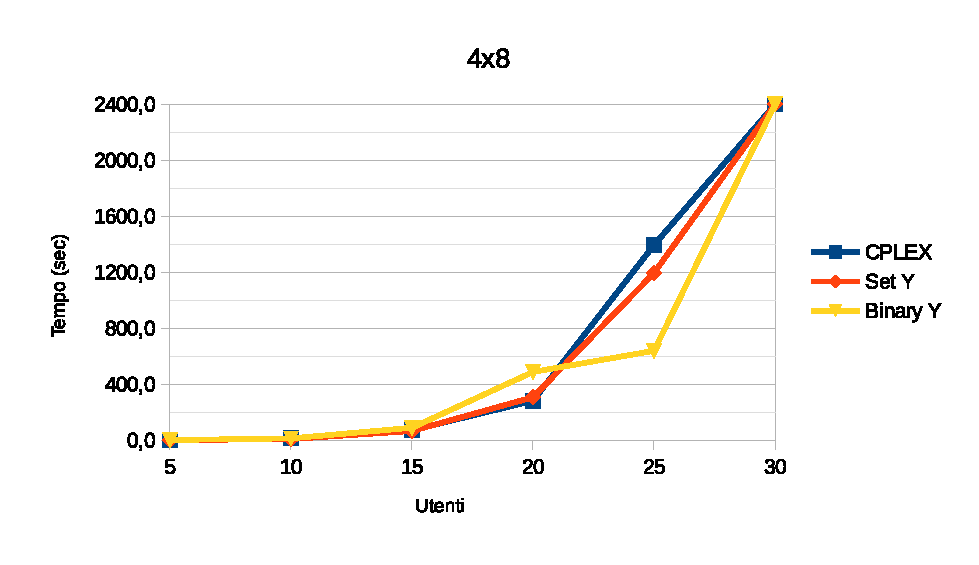
\includegraphics[scale= 0.4]{4x8.eps}
		\caption{4x8}
		\label{fig:4x8}
	\end{subfigure}
	%
	%
	\begin{subfigure}[b]{0.4\textwidth}
		\centering
		\includegraphics[scale= 0.4]{9x9.eps}
		\caption{9x9}
		\label{fig:9x9}
	\end{subfigure}
	%
	\begin{subfigure}[b]{0.4\textwidth}
		\centering
		\includegraphics[scale= 0.4]{8x20.eps}
		\caption{8x20}
		\label{fig:8x20}
	\end{subfigure}
	\caption{Confronto tempi CPLEX - euristiche}
	\label{fig:mix}
\end{figure}
%
\clearpage
%
\begin{figure}
	\begin{center}
		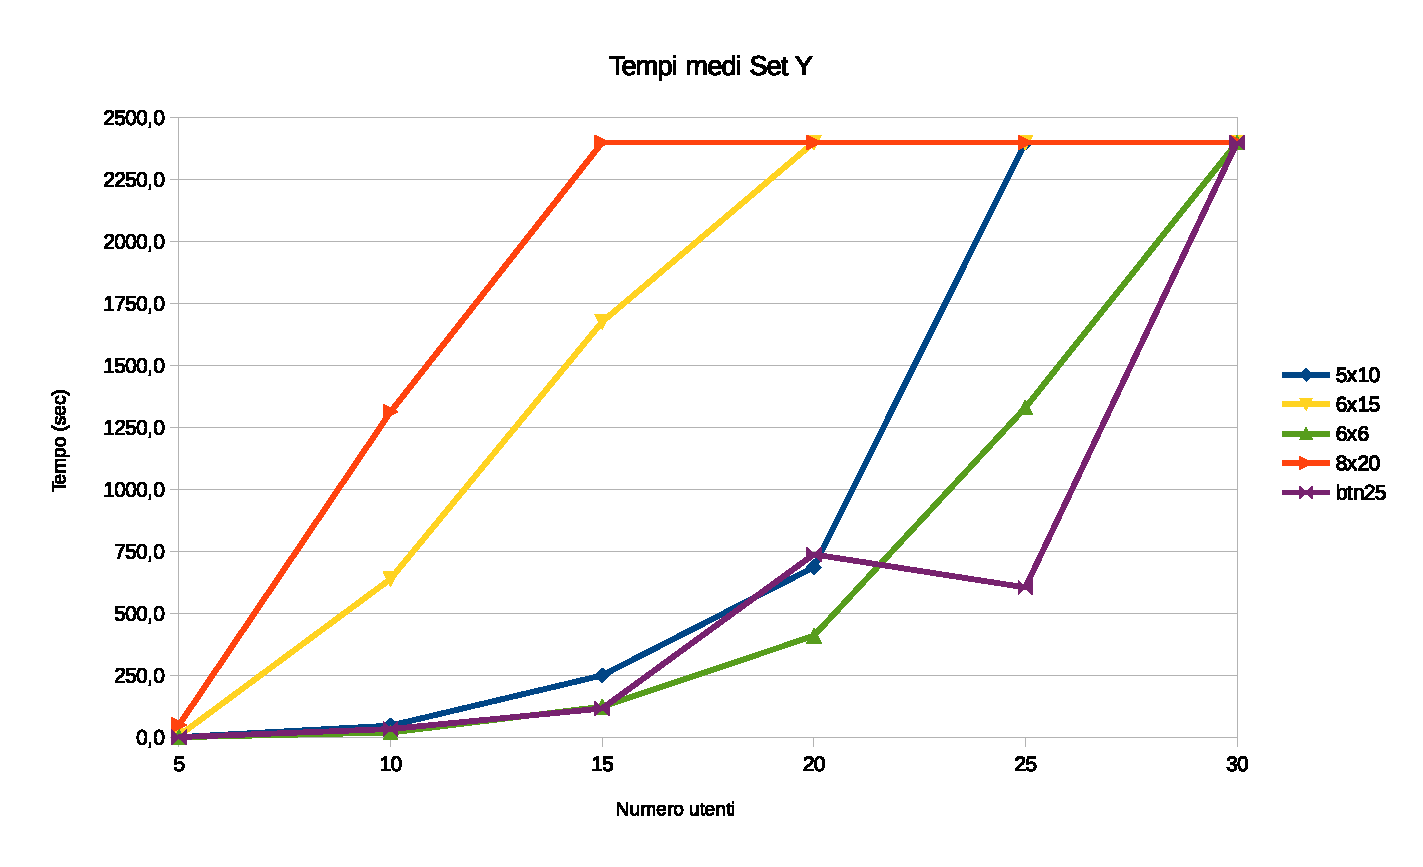
\includegraphics[width=\textwidth]{avgtimebygridSetY.eps}
	\end{center}
	\caption{Numero medio di droni per griglia} \label{fig:avgtimebygridSetY}
\end{figure}
%
%
\begin{figure}
	\begin{center}
		\includegraphics[width=\textwidth]{avgtimebygridBinaryY.eps}
	\end{center}
	\caption{Numero medio di droni per griglia} \label{fig:avgtimebygridBinaryY}
\end{figure}
%
%
\begin{figure}
	\begin{center}
		\includegraphics[width=\textwidth]{avgdrn.eps}
	\end{center}
	\caption{Numero medio di droni per griglia} \label{fig:avgdrn}
\end{figure}
%

%
\begin{figure}
	\begin{center}
		\includegraphics[width=\textwidth]{avgtime.eps}
	\end{center}
	\caption{Numero medio di droni per griglia} \label{fig:avgtime}
\end{figure}
%
